\documentclass{article}

%Added this for math
\usepackage{amsmath}
\usepackage{amssymb}
\usepackage{graphicx}
\usepackage{graphics}
\usepackage{multirow}
\usepackage{multicol}
\usepackage{epsfig}
\usepackage[table,xcdraw,svgnames,dvipsnames]{xcolor}

\usepackage{tikz}
\usepackage{pgfplots}
\usepackage{subcaption}
\pgfplotsset{compat=1.18}

\usetikzlibrary{positioning}

% ---------------------------------

	\def\papertitle{Generating Synthetic Vehicle Data Using Decentralized Generative Adversarial Networks (T-IV-23-08-2576)}
	\def\authors{B.~Shaker, G.~P.~Rosati~Papini, M.~Saveriano, and K.-Y.~Liang}
	
	\def\Editor{Dear Professor Fei-Yue Wang, Editor-in-Chief}
	
	\def\Letter{
 %I hope this message finds you well. 
 I would like to express my gratitude for your prompt response and the feedback provided by the reviewers. While I understand that there are some concerns raised by one of the reviewers, I would like to kindly request your reconsideration of our manuscript, "Generating Synthetic Vehicle Data Using Decentralized Generative Adversarial Networks," T-IV-23-08-2576, for publication in the IEEE Transactions on Intelligent Vehicles.

I would like to bring to your attention a few points that could warrant a reconsideration. 
Notably, one of the reviewers recommended acceptance after minor revisions, indicating that there is significant merit in our work that aligns with the journal's objective and scope. The second reviewer, while critical, raised points that we believe we can successfully address to meet the journal's standards. We have taken the reviewers' comments seriously and have made several revisions to address their concerns. %While we value their input, it's worth noting that some of these reviewer raised issues could have been brought up during the first review round.
We have significantly improved the manuscript based on the feedback received from the reviewers. We have achieved this by incorporating relevant references and enhancing both the clarity and the scope of the paper, in line with the request of Reviewer~2. Reviewer~2 has pointed out concerns regarding the novelty of our paper. However, the articles referenced by the reviewer do not contain material comparable to what we have presented in our paper. More in details:%Here is a breakdown of the works and their differences:
\begin{itemize}
\item \emph{Adaptive region pooling for object detection} and \emph{Adaptive pooling in multi-instance learning for web video annotation} use adaptive pooling in Convolutional Neural Networks (CNNs) for videos, without involving Federated Learning (FL), Generative Adversarial Networks (GANs), or time-series data. Our approach extends the use of CNNs to handle time-series data in a FL settings, which is a distinct contribution. 
\item \emph{Asap: Adaptive structure aware pooling for learning hierarchical graph representations} utilizes adaptive pooling for graph neural networks, which is different from our approach that uses FL, GANs, and time-series data.
\item \emph{A deep learning CNN architecture applied in smart near-infrared analysis of water pollution for agricultural irrigation resources} is the only referenced work that involves time-series data. However, it does not deal with GAN or FL.
\end{itemize}
It is important to emphasize that none of the referenced works are situated within the context of intelligent vehicles, which further underscores the unique contribution of our paper in this specific domain.

%This indicates that our work may offer a unique and innovative approach to generating synthetic data while considering privacy concerns.
%Finally, in your initial email, you expressed that you found the topic of our paper interesting and beneficial to the Transactions on Intelligent Vehicles. We believe that with the revisions we have made, the paper aligns more closely with your vision for the journal.

In light of these points, I kindly request that you reconsider our manuscript for publication. We are willing to make any necessary revisions to address the concerns raised by the reviewers and ensure that the paper meets the high standards of the IEEE Transactions on Intelligent Vehicles.

Thank you for your time and consideration.

Best regards,

Prof. Rosati Papini Gastone Pietro
}


\providecommand{\lettertitle}{Author Response to Reviews of}
\providecommand{\papertitle}{Title}
\providecommand{\authors}{Authors}
\providecommand{\journal}{Journal}
\providecommand{\doi}{--}
\providecommand{\Editor}{Name}
\providecommand{\Letter}{Body}

\usepackage[includeheadfoot,top=10mm, bottom=10mm, footskip=2.5cm]{geometry}


% Typography
\usepackage[T1]{fontenc}
\usepackage{times}
%\usepackage{mathptmx} % math also in times font
\usepackage{amssymb,amsmath}
\usepackage{microtype}
\usepackage[utf8]{inputenc}
\usepackage{bm,times} % assumes new font selection scheme installed

% Misc
\usepackage{graphicx}
\usepackage[hidelinks]{hyperref} %textopdfstring from pandoc
\usepackage{soul} % Highlight using \hl{}

\usepackage{caption}
\usepackage{subcaption}
\usepackage{graphics} % for pdf, bitmapped graphics files
\usepackage{epsfig} % for postscript graphics files
\graphicspath{{../figs/}}
\usepackage{epstopdf}
\usepackage{stfloats}

% Table

\usepackage{adjustbox} % center large tables across textwidth by surrounding tabular with \begin{adjustbox}{center}
\renewcommand{\arraystretch}{1.5} % enlarge spacing between rows
\usepackage{caption} 
\captionsetup[table]{skip=10pt} % enlarge spacing between caption and table
\usepackage{multirow}
\usepackage{booktabs}
% Section styles

\usepackage{titlesec}
\titleformat{\section}{\normalfont\Large}{\makebox[0pt][r]{\bf \thesection.\hspace{4mm}}}{0em}{\bfseries}
\titleformat{\subsection}{\normalfont}{\makebox[0pt][r]{\bf \thesubsection.\hspace{4mm}}}{0em}{\bfseries}
\titlespacing{\subsection}{0em}{1em}{-0.3em} % left before after

% Paragraph styles

\setlength{\parskip}{0.6\baselineskip}%
\setlength{\parindent}{0pt}%


% Quotation styles
\usepackage{framed}
\let\oldquote=\quote
\let\endoldquote=\endquote
\renewenvironment{quote}{\begin{fquote}\itshape\advance\leftmargini -2.4em\begin{oldquote}}{\end{oldquote}\end{fquote}}

%\usepackage{xcolor}
%\newenvironment{fquote}
%  {\def\FrameCommand{
%	\fboxsep=0.6em % box to text padding
%	\fcolorbox{blue}{white}}%
%	% the "2" can be changed to make the box smaller
%    \MakeFramed {\advance\hsize-2\width \FrameRestore}
%    \begin{minipage}{\linewidth}
%  }
%  {\end{minipage}\endMakeFramed}

\usepackage{xcolor}
\newenvironment{fquote}
{\def\FrameCommand{
		\fboxsep=0.6em % box to text padding
		\fcolorbox{blue}{white}}%
	% the "2" can be changed to make the box smaller
	\MakeFramed {\advance\hsize-3\width \FrameRestore}
	}
	{\endMakeFramed}

% Table styles

\let\oldtabular=\tabular
\let\endoldtabular=\endtabular
\renewenvironment{tabular}[1]{\begin{adjustbox}{center}\begin{oldtabular}{#1}}{\end{oldtabular}\end{adjustbox}}


% Shortcuts

%% Let textbf be both, bold and italic
%\DeclareTextFontCommand{\textbf}{\bfseries\em}

%% Add RC and AR to the left of a paragraph
%\def\RC{\makebox[0pt][r]{\bf RC:\hspace{4mm}}}
%\def\AR{\makebox[0pt][r]{AR:\hspace{4mm}}}

%% Define that \RC and \AR should start and format the whole paragraph 

\newcounter{RCcounter}
\setcounter{RCcounter}{0}
\newcounter{Rcounter}
\setcounter{Rcounter}{0}

\usepackage{suffix}
\long\def\RC#1\par{\makebox[0pt][r]{\bf RC\arabic{Rcounter}\arabic{RCcounter}:\hspace{4mm}}\textbf{{#1}}\par} %\RC
\WithSuffix\long\def\RC*#1\par{\textbf{{#1}}\par} %\RC*
\long\def\AR#1\par{\makebox[0pt][r]{AR\arabic{Rcounter}\arabic{RCcounter}:\hspace{10pt}}{\textcolor{blue}{#1}}\stepcounter{RCcounter}\par} %\AR
\WithSuffix\long\def\AR*#1\par{{#1}\par} %\AR*


\def\headall{
\setcounter{RCcounter}{1}
{\Large\bf \lettertitle}\\[1em]
{\Large \papertitle}\\[1em]
{\authors}\\
%{\it \journal, }\texttt{doi:\doi}\\
\hrule
% Legend
\hfill {\bfseries RC:} \textbf{{Reviewer Comment}},\(\quad\) AR: \textcolor{blue}{Author Response}, \(\quad\textcolor{blue}{\square}\) \emph{\textcolor{blue}{Manuscript text}}
\stepcounter{Rcounter}}


%%%
%DIF PREAMBLE EXTENSION ADDED BY LATEXDIFF
%DIF UNDERLINE PREAMBLE %DIF PREAMBLE
\RequirePackage[normalem]{ulem} %DIF PREAMBLE
\RequirePackage{color}\definecolor{RED}{rgb}{1,0,0}\definecolor{BLUE}{rgb}{0,0,1} %DIF PREAMBLE
\providecommand{\DIFadd}[1]{{\protect\color{blue}\uwave{#1}}} %DIF PREAMBLE
\providecommand{\DIFdel}[1]{{\protect\color{red}\sout{#1}}}                      %DIF PREAMBLE
%DIF SAFE PREAMBLE %DIF PREAMBLE
\providecommand{\DIFaddbegin}{} %DIF PREAMBLE
\providecommand{\DIFaddend}{} %DIF PREAMBLE
\providecommand{\DIFdelbegin}{} %DIF PREAMBLE
\providecommand{\DIFdelend}{} %DIF PREAMBLE
%DIF FLOATSAFE PREAMBLE %DIF PREAMBLE
\providecommand{\DIFaddFL}[1]{\DIFadd{#1}} %DIF PREAMBLE
\providecommand{\DIFdelFL}[1]{\DIFdel{#1}} %DIF PREAMBLE
\providecommand{\DIFaddbeginFL}{} %DIF PREAMBLE
\providecommand{\DIFaddendFL}{} %DIF PREAMBLE
\providecommand{\DIFdelbeginFL}{} %DIF PREAMBLE
\providecommand{\DIFdelendFL}{} %DIF PREAMBLE
%DIF END PREAMBLE EXTENSION ADDED BY LATEXDIFF

% Highlight
\newcommand{\highlight}[2][yellow]{\mathchoice%
	{\colorbox{#1}{$\displaystyle#2$}}%
	{\colorbox{#1}{$\textstyle#2$}}%
	{\colorbox{#1}{$\scriptstyle#2$}}%
	{\colorbox{#1}{$\scriptscriptstyle#2$}}}%

 \usepackage{pdfpages}
 
\newcommand{\sqboxEmpty}[1]{%
	\colorbox{#1}{\Square}%
}%


\begin{document}
{\Large\bf \Editor}\\[1em]
{\large\Letter}\\[1em]
%\newpage
% Make title
\headall


%\section{Editor}
%\RC fdf\\

%\AR dsadas
%\RC Reviewer Comments concerning your manuscript, "Generating Synthetic Vehicle Data Using Decentralized Generative Adversarial Networks," T-IV-23-08-2576, have been obtained and are copied below. Based on the attached reviewers' comments, we will not be able to publish your manuscript in our transactions.

%I believe the topic of your paper is interesting and beneficial to TIV, therefore I would like to invite you to revise thoroughly according to our review reports, and resubmit your revision as a New paper. If you do so, please let me know before your submission and provide me with a detailed report on your revision, I will let you know my opinion.

%\AR TODO
%\RC comment

%\AR Please refer to the individual reviewer replies for details.


%\newpage
% Make title
%\headall

%\newpage
%\headall

\section{Reviewer \#1}

\RC The author revised most of my suggestions and the paper can be accepted after minor revisions. \\

\AR Thank you for your valuable feedback and your thorough review of our paper. We greatly appreciate your time and effort in providing us with insightful suggestions for improvement. We are grateful for your evaluation and are pleased to hear that the paper can be accepted with only minor revisions.

\RC For instance, the discussion on the latest review articles in the field of scenarios and related articles was missing in the present article. I suggest discussing the following and similar articles in the literature review section.
\begin{itemize}
	\item From Features Engineering to Scenarios Engineering for Trustworthy AI:I\&I,C\&C, and V\&V. (IEEE IS)
	\item ParallelEye Pipeline: An Effective Method to Synthesize Images for Improving the Visual Intelligence of Intelligent Vehicles (IEEE SMC-Systems)
	\item A Novel Scenarios Engineering Methodology for Foundation Models in Metaverse (IEEE SMC-Systems)
\end{itemize}

\AR Thank you for your feedback and the valuable suggestions for improving our paper. We appreciate your effort in providing us with specific references that can enhance our literature review section. We have incorporated a discussion of the mentioned articles in our revised version to provide a more comprehensive overview of the field. \newline
We added the following text in the revised version of the manuscript.

\begin{quote}
A possible solution consists in using synthetic data like images [1].
    \newline\newline
    Moreover, we will investigate the possibility to
make our model explainable relying on approaches from
scenario engineering [22], [23].
\end{quote}

\newpage
\headall

\section{Reviewer \#2}

\RC The title of this manuscript is not specific enough. Considering that there are many kinds of data within the vehicles, what the data is denoted for should be clarified in the title. 

\AR Thank you for taking the time to provide feedback on our manuscript's title. We genuinely appreciate your input and have carefully considered your suggestion. As outlined in the main body of the paper, the data predominantly originates from the APS system. However, it is important to note that our approach is designed to be applicable to a broader range of time-series data, encompassing both discontinuous and continuous types. We recognize the importance of clarity in the title but must also balance this with the need to avoid overly narrowing the scope, especially since the data in the paper is anonymized for privacy reasons. 
In light of these considerations, we remain open to revisiting the title if you believe it is necessary to further clarify the scope.

%\AR Thank you for your suggestion. How is written in the main body of the paper the data come from the APS system, however the approach is general and can work for different time-series data. Indeed the time-series data are both of discontinuous or continuous nature. Specify the type of data in the title narrows down the scope of this paper, moreover the data are anonymized in the text for privacy reasons. 

\RC The novelty of this paper is limited. Only very basic GAN and FL training approaches are adopted, which can hardly meet the standards of T-IV. CNN with adaptive pooling layers has been widely exploited in recent works. 

\AR We appreciate your concerns and would like to provide you with a detailed list of our main contributions.
\begin{itemize}
	\item We acknowledge that the use of GAN in conjunction with Federated Learning (FL) for time series data may initially seem to adopt basic approaches. However, it's important to note that the comprehensive exploration of GAN with Federated Learning in the context of time series data has not been extensively covered in the existing literature (moreover in the context of vehicle data). In our study, we benchmark our approach against TimeGAN, which is one of the most similar methods available, but it does not incorporate FL. This comparison highlights our unique contribution within this specific context.
	\item We understand that the use of Convolutional Neural Networks (CNN) with adaptive pooling layers has become prevalent in recent works. However, our contribution lies in the adaptation of these layers specifically to accommodate time series data. This adaptation is a critical aspect of our research and distinguishes it from most applications of CNN layers in other domains.
	\item In our work, we also address the issue of data normalization techniques, modifying them to suit the FL context (Figure 6). This adaptation further enhances the applicability and effectiveness of our approach in FL scenarios.
\end{itemize}
It's worth noting that the recommended papers you mentioned primarily focus on image-related applications. While one of them discusses time series data, it doesn't pertain to the FL context or the use of GAN, which underscores the novelty of our research in bridging these techniques within a time-series domain using vehicle data.\\
We value your feedback, and we hope these explanations shed light on the significance of our research within the presented context.

%\AR 
%1. GAN e FL non è mai stato testato per time-series.
%2. e c'è una modifica degli algotitmi per essere adattati alle time-series (abbiamo fatto discrimitor)
%Tantè che i paper citati o usano le immagini o ppure utilizzano altre artchitetture rispetto alle gan.
%CNN utilizzano le adaptive pooling layer ma su immagini noi lo stuamo facendo su time-series.

\RC The experiments are not comprehensively conducted. On the one hand, no recent and related FL-based GANs are compared on the same tasks, on the other hand, the ablation studies are missing. Detailed analysis of the components of each part should be conducted. 

\AR Thank you for your feedback, we appreciate the opportunity to clarify the methodology and rationale behind our choices: \newline\newline
%\begin{description}
	\textbf{Ablation Studies:} We acknowledge the importance of ablation studies in evaluating the components of our approach. However, please note that the ablation study we conducted was performed on image data and has been thoroughly documented in response to previous reviewers' comments. For completeness, we have included that response at the end of this reply. While ablation studies are valuable, they often require a substantial amount of space to be explained in detail, which could have diverted attention from our primary research objectives. Moreover due to space constraints, we aimed to prioritize presenting our work on time series data. 
	This focus was intended to provide a clear and detailed account of our contributions within the scope of this specific research context.
 \newline\newline
	\textbf{Comparison with Recent FL-based GANs:} We understand your concern about the comparison with recent Federated Learning-based GANs. In our evaluation, we have compared our approach primarily with TimeGAN, which is a relevant benchmark in the context of time series data generation. We want to emphasize that, as of our knowledge cutoff date in September 2021, there were limited FL-based GANs specifically designed for time series data. Therefore, we believe our choice of comparison with TimeGAN is fair given the available literature. We sincerely value your additional recommendations for the bibliography; however, none of the presented works aligns with our specific research objectives."
%\end{description}
\newline\newline
\textbf{The Ablation Study on Images}
\newline\newline
To realise a work with these characteristics, an ablation studies is a must. For this reason, we conducted a series of preliminary ablation studies specifically for image-based GANs before adapting it to time-series data. In particular we studied:
\begin{itemize}
	\item The effects of different loss functions, particularly MSE and BCE. In a centralized setup, there were no major difference between the performance of BCE and MSE loss, however, MSE performed significantly better than BCE. 
 \colorlet{myblue}{gray!60!blue}
\colorlet{msecol}{orange}

\def\bcescale{0.8}
\def\bceyscale{0.5}
\def\bcecol{myblue}

\begin{figure}[htp]
    \centering
    \begin{subfigure}[b]{0.45\textwidth}
        \centering
        \begin{tikzpicture}[scale=\bcescale]
            \begin{axis} [
                xlabel={Training Step},
                ylabel={FID Score},
                axis x line=bottom,
                axis y line*=left,
                yticklabels={},
                line width=2pt,
xtick={0,5000,10000,15000,20000,25000,30000},
xticklabels={0,5k, 10k, 15k, 20k, 25k,30k},
scaled ticks=false,
                ]
                \addplot[\bcecol, line width=2pt] table [col sep=comma,header=true,x index=3,y index=4] {Reply_to_comments_v2/bce-mse-smooth.csv};
                \addplot[msecol, line width=2pt] table [col sep=comma,header=true,x index=3,y index=5] {Reply_to_comments_v2/bce-mse-smooth.csv};
                \legend{BCE Loss, MSE Loss}
            \end{axis}
        \end{tikzpicture}
        \caption{One worker centralized result}
    \end{subfigure}
    \hfill
    \begin{subfigure}[b]{0.45\textwidth}
        \centering
        \begin{tikzpicture}[scale=\bcescale]
            \begin{axis} [
                xlabel={Training Step},
                ylabel={FID Score},
                axis x line=bottom,
                axis y line*=left,
                yticklabels={},
                line width=2pt,
xtick={0,5000,10000,15000,20000,25000,30000},
xticklabels={0,5k, 10k, 15k, 20k, 25k,30k},
scaled ticks=false,
                ]
                \addplot[\bcecol, line width=2pt] table [col sep=comma,header=true,x index=0,y index=1] {Reply_to_comments_v2/bce-mse-smooth.csv};
                \addplot[msecol, line width=2pt] table [col sep=comma,header=true,x index=0,y index=2] {Reply_to_comments_v2/bce-mse-smooth.csv};
                \legend{BCE Loss, MSE Loss}
            \end{axis}
        \end{tikzpicture}
        \caption{Five worker decentralized result}
    \end{subfigure}
    \caption{The FID score results of BCE vs. MSE loss}
    \label{fig:bce-mse}
\end{figure}

	\item The impact of batch size on the performance of the image-based GANs. The network was able to learn much faster using a smaller batch size of 16 compared to 64. Both the image output and the FID score confirm that the output improved with a smaller size batch given a larger number of workers and limited local data.
 
\colorlet{myblue}{blue!50}
\colorlet{orange}{orange}

\def\batchscale{0.6}
\def\batchyscale{0.45}
\def\batchcol{myblue}
\def\batchtcol{orange}

\begin{figure}[htp]
    \centering
    \begin{subfigure}[b]{0.45\textwidth}
        \centering
        \begin{tikzpicture}[label distance=-3mm]
            \clip(-1.8,-2.7) rectangle (6.1,2);
            \node[inner sep=0pt,label={below:Batch Size = 64}] (sixty) at (0,0)
                {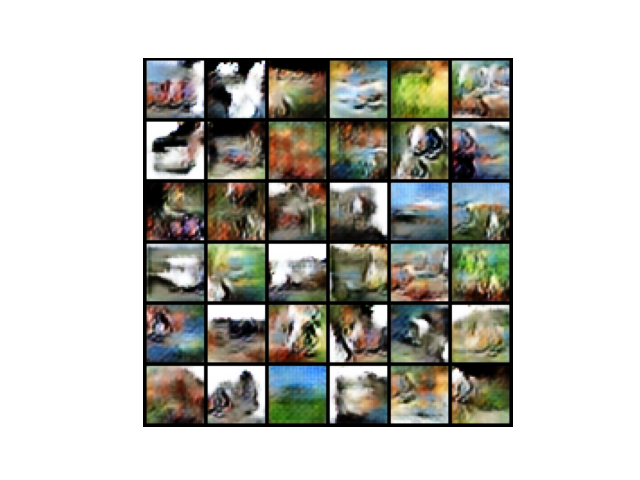
\includegraphics[scale=0.4]{Reply_to_comments_v2/images/64-30.png}};
            \node[inner sep=0pt,right = -2.4 cm of sixty,label={below:Batch Size = 16}] (sixteen)
                {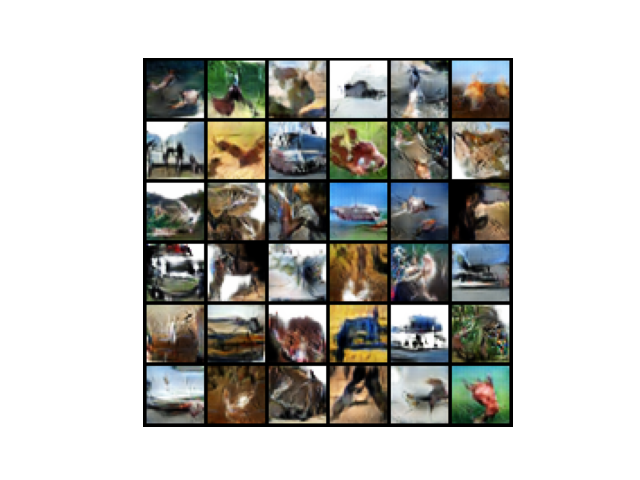
\includegraphics[scale=0.4]{Reply_to_comments_v2/images/16-30.png}};
        \end{tikzpicture}
        \caption{Output at 30 epochs}
    \end{subfigure}
    \hfill
    \begin{subfigure}[b]{0.45\textwidth}
        \centering
        \begin{tikzpicture}[scale=\batchscale]
            \begin{axis} [
                xlabel={Training Step},
                ylabel={FID Score},
                ylabel near ticks,
                ylabel shift=-10pt,
                axis x line=bottom,
                axis y line*=left,
                yticklabels={},
xtick={0,5000,10000,15000,20000,25000,30000},
xticklabels={0,5k, 10k, 15k, 20k, 25k,30k},
scaled ticks=false,
                line width=2pt
                ]
                \addplot[\batchcol, line width=2pt] table [col sep=comma,header=true,x index=0,y index=1] {Reply_to_comments_v2/batch-size-smooth.csv};
                \addplot[\batchtcol, line width=2pt] table [col sep=comma,header=true,x index=0,y index=2] {Reply_to_comments_v2/batch-size-smooth.csv};
                \legend{Batch Size 64, Batch Size 16}
            \end{axis}
        \end{tikzpicture}
        \caption{FID score comparison}
    \end{subfigure}
    \caption{The batch size effect on performance for the image-based GAN model}
    \label{fig:batch-size}
\end{figure}
	\item The effect of the learning rate on the weighted average of the most and least forgiving strategies. We experimented with different learning rates for the discriminator and generator, specifically increasing the discriminator learning rate to 0.002. Additionally, we adjusted the discriminator-generator training ratio to 3:1. Despite these modifications, the changes resulted in image output degradation.
\end{itemize}
Obviously, these tests carried out on image-based GANs have been omitted for reasons of space in the final discussion, limiting ourselves to presenting the final studies carried out directly on time-series more in detail as more interesting and specific in our work.
In particular we report:
\begin{itemize}
	\item The effect of the dynamic window reported in Table~II.
	\item The effect of worker normalization, Table~III.
	\item The effect of Federated Learning strategy, Table~IV.
\end{itemize}

%\AR Tutto ablation study è stato svolto su immagini e è riportato in modo esaustivo nella risposta ai revisori. Il confronto è stato fatto su TimeGan del 2019. Nella bibliografia proposta non sono stati consigliati nessun FL-based GANs.

\RC The use of CNN with an adaptive pooling mechanism should be compared with the traditional CNN methods in the experiments.

\AR We truly appreciate your suggestion. We would like to clarify that this comparison is already incorporated into our paper, specifically in Table 2, which illustrates the "dynamic window effect." It's worth noting that the adaptive pooling layer is exclusively included in the "dynamic window" architecture. In contrast, the fixed windows (64 -> 256) do not utilize the adaptive pooling layer, allowing for a direct comparison to assess the impact of this specific pooling layer. Moreover,  the adaptive pooling layer is only applicable to time-series, as it was not needed previously for image based tests.

%\AR This is already included in the paper, its table 2 (dynamic window effect). The adaptive pooling layer is only included in the "dynamic window" architecture. The fixed windows 64 -> 256 dont have the adaptive pooling layer, which means this is a direct comparison to find the effect of the pooling layer. There are mentions in the text why we have included it, but I guess we need to be very explicit in saying that under the results for table 2. Another thing is the adaptive pooling layer is only applicable to time-series, as it was not needed previously for image based.

\RC Different normalization methods should be discussed and compared in the experiments such as layer normalization, group normalization, and batch normalization.

\AR  Thank you for your suggestion. In our study, we employed two specific normalization techniques: batch normalization on the generator side and spectral normalization on the discriminator side. These choices were influenced by prior research, particularly the work on F2U and F2A, which served as the foundation for our research. During the initial stages of our experimentation and in our efforts to replicate their findings, we observed that spectral normalization was crucial for the discriminator. Without it, the discriminator failed to yield meaningful results. While we understand the value of exploring different normalization methods, we also considered the substantial body of existing research that has already established the effectiveness of these specific techniques in the context of our work. 

%\textcolor{red}{Could some numerical results be added that validate our approach?}

%TODO can we present results to support our choice?

%TODO add in the text that we tested different types of normalisation by verifying what had been presented in work X.

%\AR So there are 2 normalization techniques that we used. batch norm on the generator side, and spectral norm on the discriminator side. This was based upon the previous work done on F2U and F2A in the main paper this was built upon. During the early stages of my testing and recreating their work, it was apparent that the discriminator needed to have spectral norm vs. batch norm, as without it, it never gave any results. In my mind, I feel like we don't need to redo work that has been previously established.
% AGGIUNGERE UNA FRASE nel testo del paper che abbiamo testato differenti tipi di normalizzazione.

\RC I understand that the authors deleted some fundamental knowledge for the introduction part in the revised manuscript, however, more elaboration on the motivation of the proposed method should be added. Why do we need such a method? What problems are solved with these methods? Why existing methods fail to provide a solution to these problems.

\AR We appreciate your feedback regarding the motivation behind our proposed method. Your input has been instrumental in enhancing the clarity of our research, and we have taken your comments to heart.
We have taken steps to provide more detailed elaboration on the motivation for our method. Specifically, our approach enables the generation of vehicle-data while respecting privacy by avoiding centralized data sharing. Within our context, this data is instrumental in replicating anomalous vehicle behaviors, serving the purpose of identifying potential malfunctions, all without the need for data sharing.
By incorporating these additional details, we aim to offer a clearer understanding of why our method is necessary and how it addresses key challenges. We hope that these revisions make the motivation behind our research more evident and compelling.
Your valuable feedback continues to guide the improvement of our manuscript, and we genuinely appreciate your constructive input.

\begin{quote}
Intelligent vehicles have the potential to revolutionize transportation by enhancing safety, efficiency, and comfort. However, developing and optimizing Machine Learning (ML) models for these vehicles requires large amounts of data. A possible solution consists in using synthetic data like images [1]. Ideally, synthetic data should be generated automatically by a generative model, like the Generative Adversarial Network (GAN) [2]. However, also generative models need to be trained on real to generated synthetic data with high fidelity.
Anonymously collecting this data is essential to protecting privacy, while ensuring that the ML models are trained on diverse and representative data to achieve good performance.
Data privacy and non-Independent and Identically Distributed (non-IID) nature of the data across vehicles pose challenges to this development. In this work, we propose a decentralized GAN model that can generate synthetic data, mimicking the behavior of local data, while preserving privacy, i.e., without sharing sensitive information
across different vehicles.
\end{quote}

%\AR Possiamo aggiungere alcune informazioni aggiungtive nell'introduzione di AGGIUNGERE UN FRASE

\RC Reference to be added:
\begin{itemize}
	\item Tsai Y H, Hamsici O C, Yang M H. Adaptive region pooling for object detection[C]//Proceedings of the IEEE Conference on Computer Vision and Pattern Recognition. 2015: 731-739.
	\item Zhou Y, Sun X, Liu D, et al. Adaptive pooling in multi-instance learning for web video annotation[C]//Proceedings of the IEEE International Conference on Computer Vision Workshops. 2017: 318-327.
	\item Ranjan E, Sanyal S, Talukdar P. Asap: Adaptive structure aware pooling for learning hierarchical graph representations[C]//Proceedings of the AAAI Conference on Artificial Intelligence. 2020, 34(04): 5470-5477.
	\item Chen H, Chen A, Xu L, et al. A deep learning CNN architecture applied in smart near-infrared analysis of water pollution for agricultural irrigation resources[J]. Agricultural Water Management, 2020, 240: 106303.
\end{itemize}

\AR Thank you for the additional references. We have added them to the Related Work section. These references are important to highlight the benefits of adaptive pooling in CNNs and graph NN. However, we would like to point out that none of the references refers to federated time-series generation, the topic of our paper. \newline
We added the following text in the revised version of the manuscript.

\begin{quote}
Both the generator and the discriminator are typically based on a Convolutional Neural Network
(CNN), a fundamental building block in deep architectures [3], that alternates between convolution and pooling layers. Having a pooling layer with fixed stride can limit the performance, therefore, adaptive pooling layers have been proposed for object detection [4], video annotation [5], and feature extraction from near-infrared spectroscopy data [6]. Adaptive pooling is also effective in learning large graph neural networks [7]. Therefore, in this work, we also exploit adaptive pooling to
train GANs on time-series data.
\end{quote}

\end{document}
